\chapter{Modeling}

\section{Introduction}
This chapter formalizes MapIT through analysis and modeling artifacts. The diagrams and schemas presented here translate the conception choices into a precise structural view of the system. They are important because they make the behavior of the application easier to verify before implementation begins.

\section{Actors and Use Cases}
The use case model identifies the principal actors of the system, such as a standard user and an administrator, and shows how each role interacts with the application. The use case diagram provides a global view of the services offered by MapIT, including authentication, incident management, document management, and administrative operations. This representation helps the reader understand the scope of the system before entering into detailed scenarios.

Figure~\ref{fig:use-case-mapit} summarizes the interactions between users and the core services of the platform.

\begin{figure}[H]
	\centering
	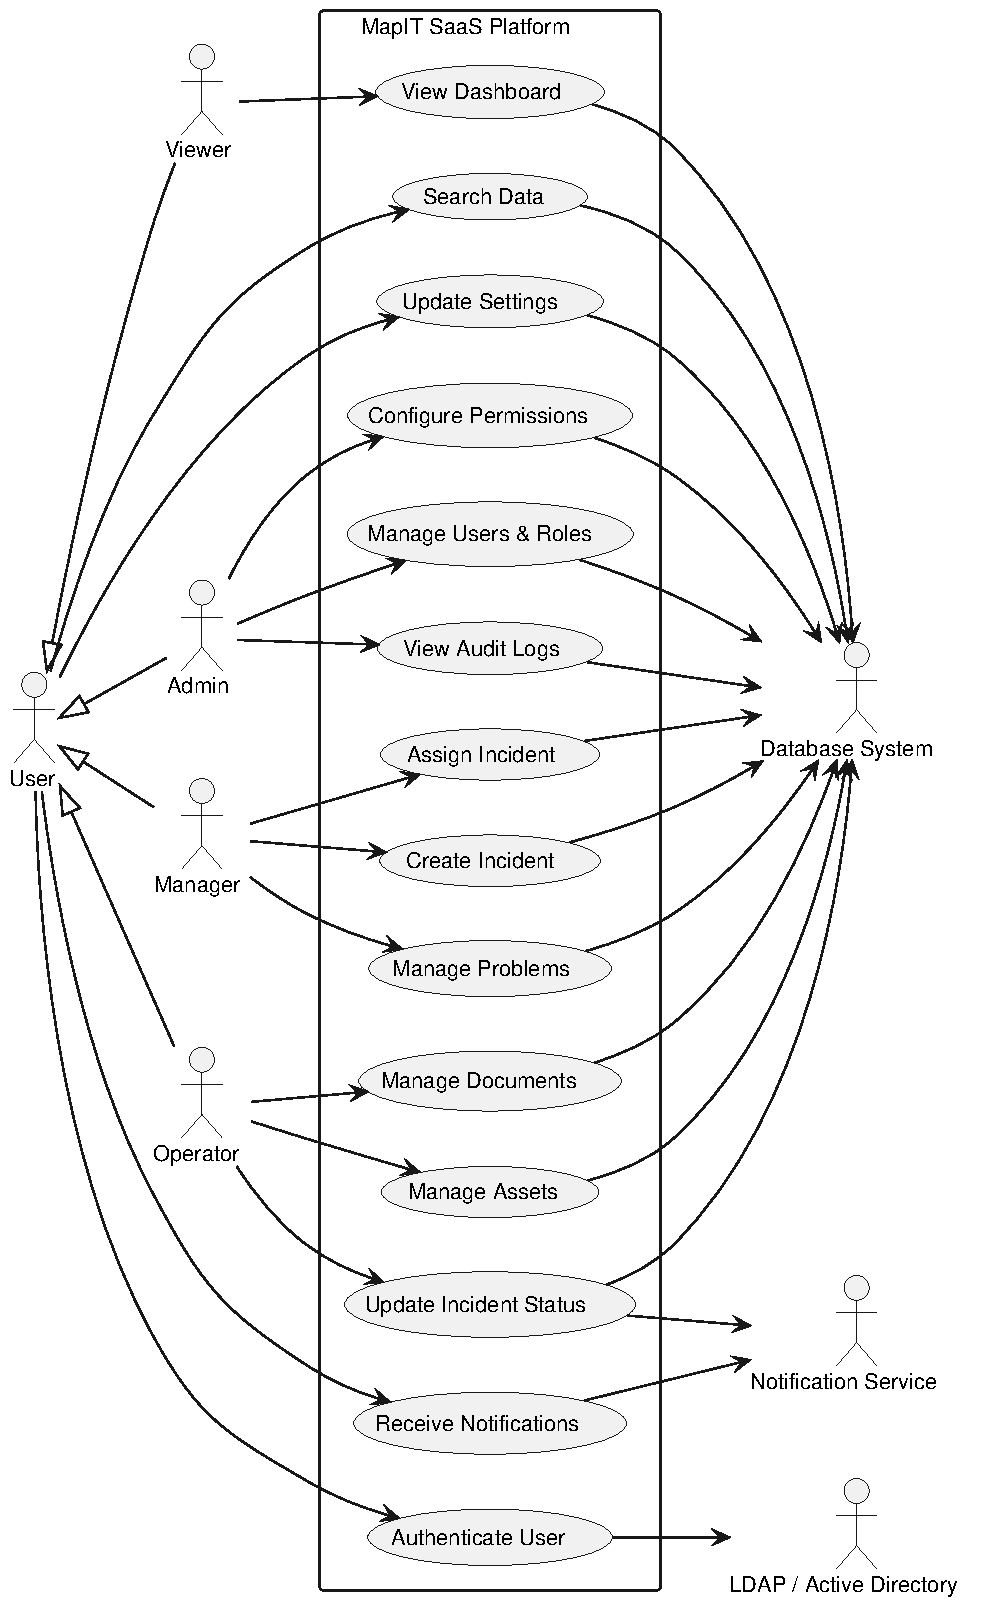
\includegraphics[width=0.92\textwidth]{figures/diagrams/updated_use_case_diagram.pdf}
	\caption{Use case diagram of MapIT}
	\label{fig:use-case-mapit}
\end{figure}

\section{Use Case Specifications}
Each major use case is described textually in terms of goal, actor, preconditions, main steps, alternate paths, and postconditions. This level of detail is important because it shows how the system behaves when a user logs in, creates a record, edits content, or performs a restricted action. The textual specification also serves as a useful reference during development and testing.

\section{Sequence Diagrams}
Sequence diagrams are used to describe the dynamic behavior of the system for representative scenarios such as authentication, incident creation, and document consultation. They show the message flow between the user interface, the API layer, the business logic, and the database, making it easier to verify that the architecture supports the intended user journeys. In an academic report, these diagrams also help demonstrate that the implementation follows a coherent interaction pattern.

The authentication interaction flow is shown in Figure~\ref{fig:seq-auth}.

\begin{figure}[H]
	\centering
	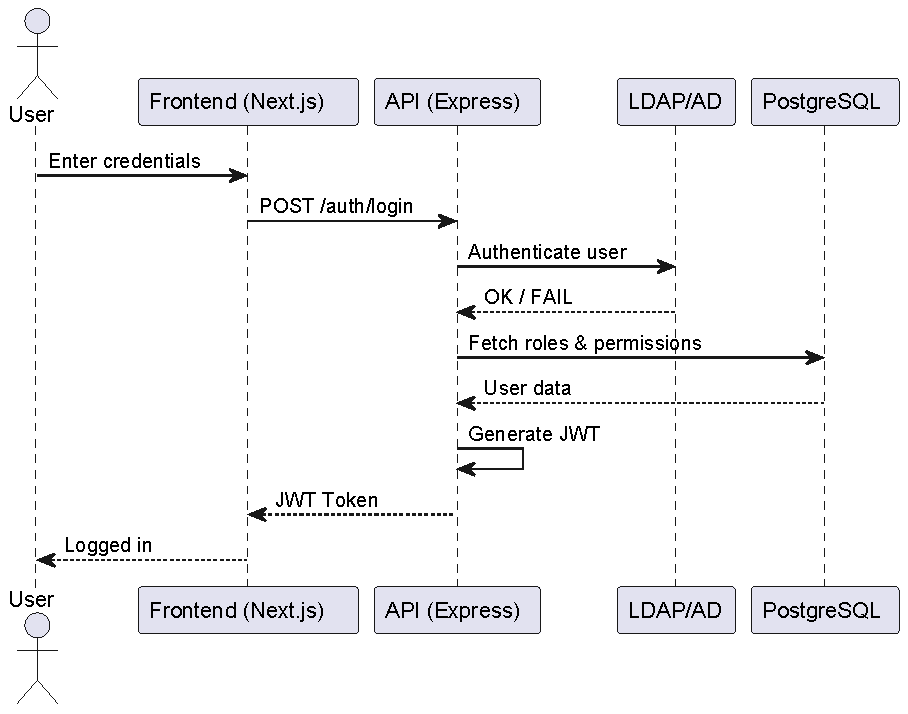
\includegraphics[width=0.95\textwidth]{figures/diagrams/sequence_diagram_authentication.pdf}
	\caption{Sequence diagram: authentication flow}
	\label{fig:seq-auth}
\end{figure}

The advanced authentication scenario, including session and permission checks, is shown in Figure~\ref{fig:seq-auth-advanced}.

\begin{landscape}
\begin{figure}[p]
	\centering
	\vspace*{\fill}
	\begin{adjustbox}{width=\linewidth, totalheight=0.8\textheight, keepaspectratio}
		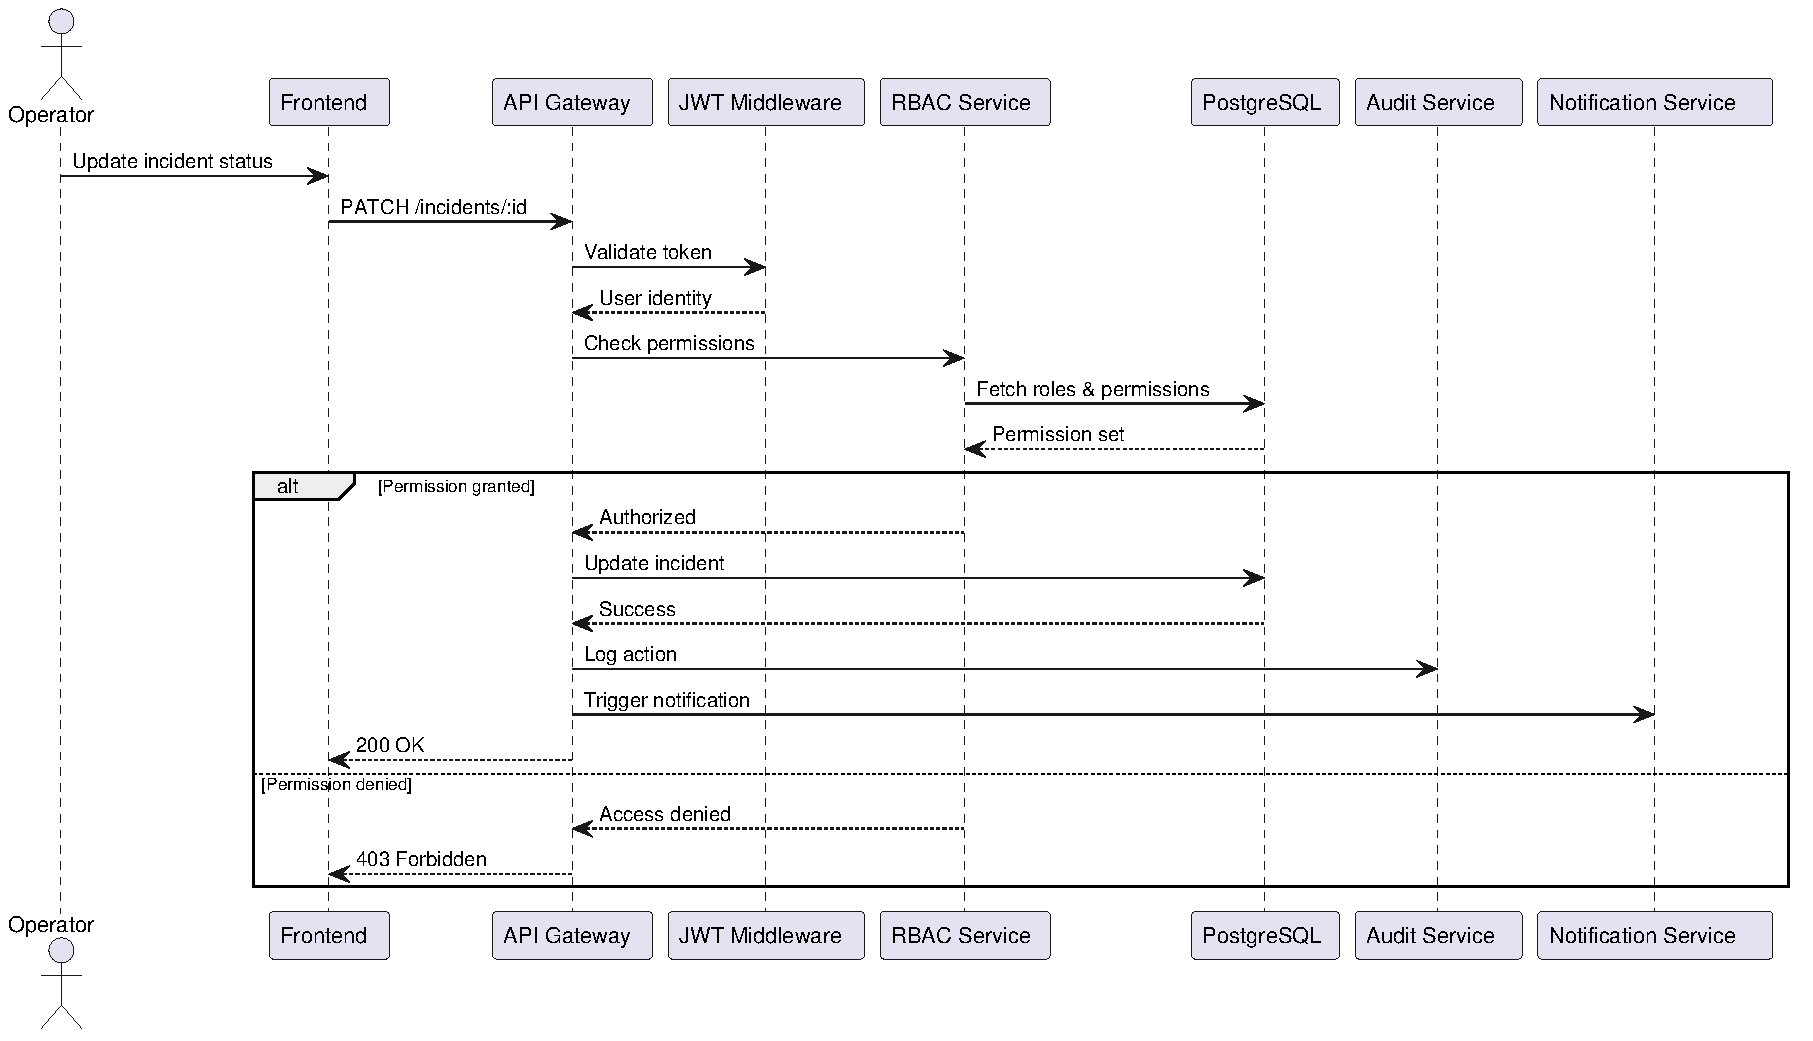
\includegraphics{figures/diagrams/advanced_auth_sequence_diagram.pdf}
	\end{adjustbox}
	\vspace*{\fill}
	\caption{Advanced authentication sequence diagram}
	\label{fig:seq-auth-advanced}
\end{figure}
\end{landscape}

The lifecycle of incident processing is detailed in Figure~\ref{fig:seq-incident}.

\begin{figure}[H]
	\centering
	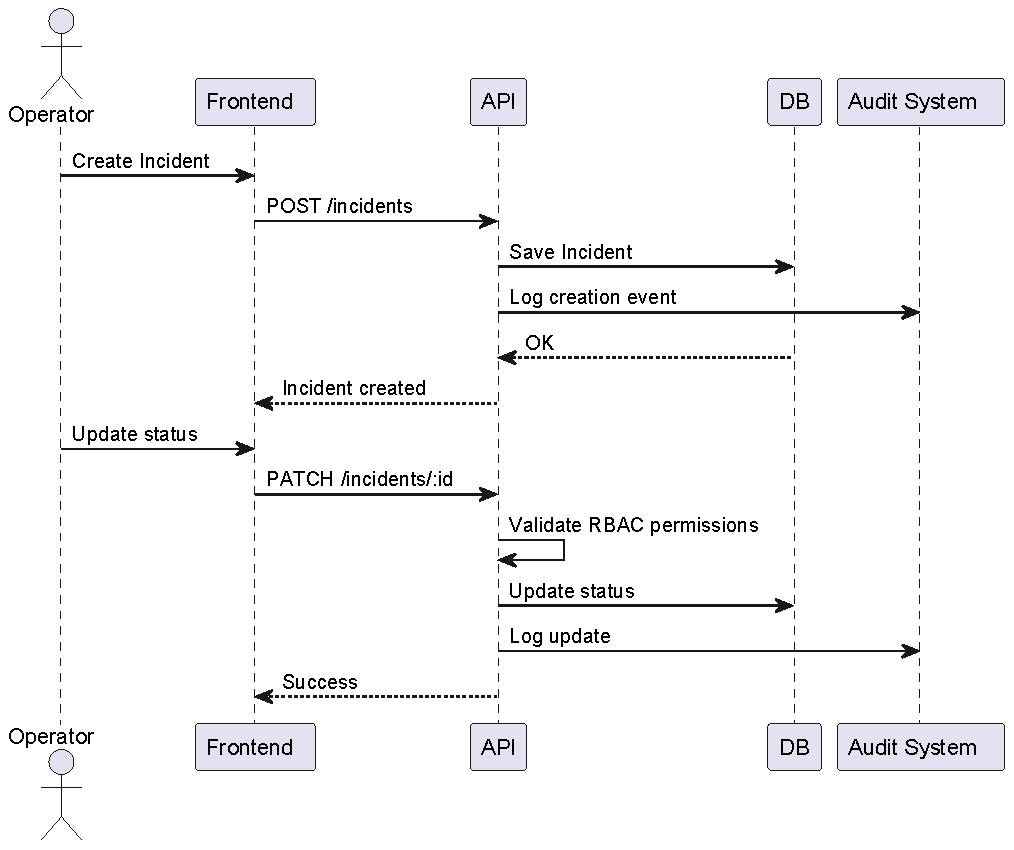
\includegraphics[width=0.95\textwidth]{figures/diagrams/sequence_diagram_incident_flow.pdf}
	\caption{Sequence diagram: incident management flow}
	\label{fig:seq-incident}
\end{figure}

The global search interaction, which aggregates multiple data domains, is presented in Figure~\ref{fig:seq-search}.

\begin{figure}[H]
	\centering
	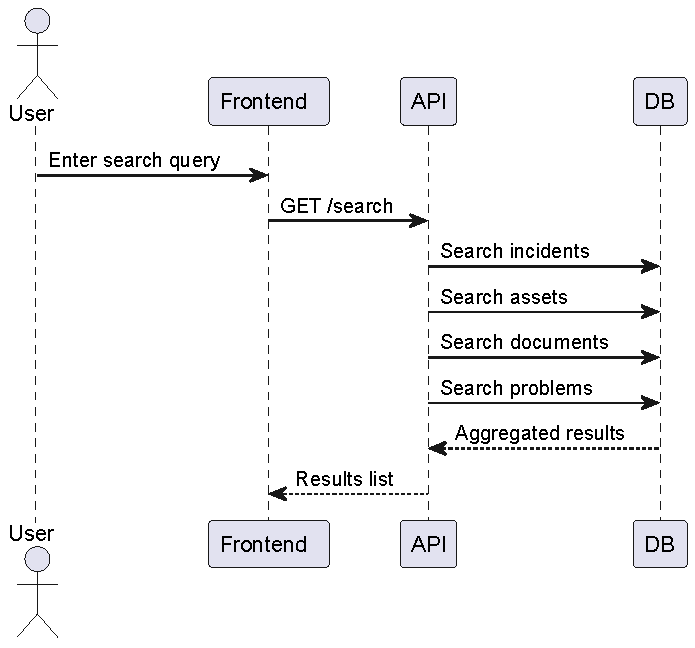
\includegraphics[width=0.95\textwidth]{figures/diagrams/sequence_diagram_global_search.pdf}
	\caption{Sequence diagram: global search flow}
	\label{fig:seq-search}
\end{figure}

\section{Class Diagram and Domain Model}
The class diagram captures the static domain structure of MapIT and presents the main entities of the application. Typical classes include User, Role, Incident, Document, Category, Comment, and AuditLog, together with the relationships that connect them. The diagram makes it clear which objects own data, which objects reference others, and how the domain supports both documentation and traceability.

Figure~\ref{fig:class-mapit} illustrates the domain model used to implement these entities and their associations.

\begin{landscape}
\begin{figure}[p]
    \centering
	\vspace*{\fill}
    \begin{adjustbox}{width=\linewidth, totalheight=0.8\textheight, keepaspectratio}
		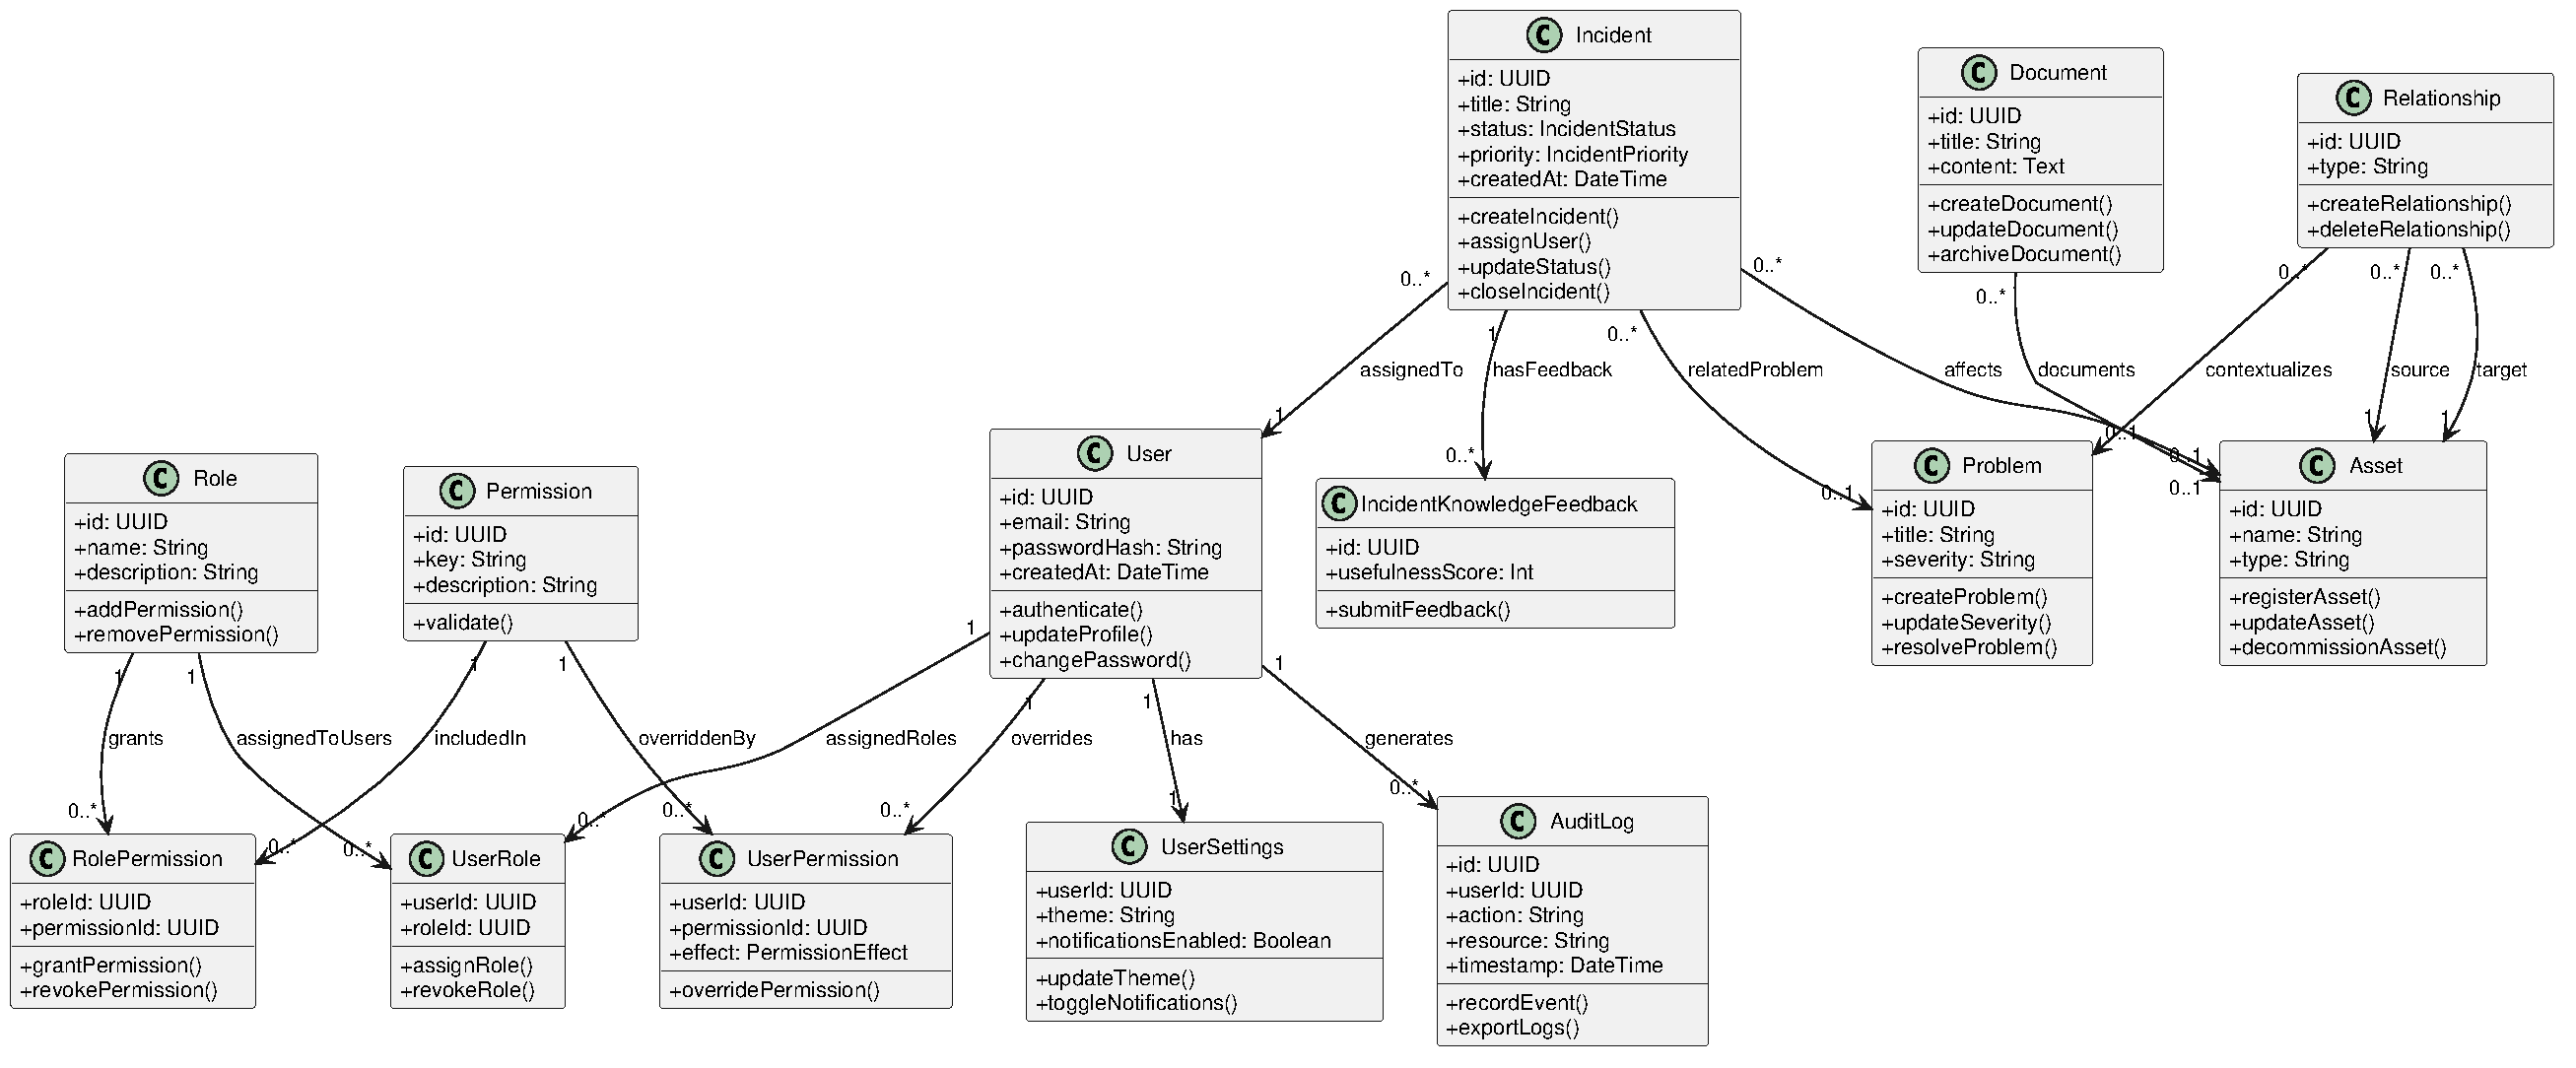
\includegraphics{figures/diagrams/updated_class_diagram.pdf}
    \end{adjustbox}
	\vspace*{\fill}
    \caption{Class diagram of the MapIT domain model}
    \label{fig:class-mapit}
\end{figure}
\end{landscape}


\section{Data Model and Relational Schema}
Once the conceptual model is established, it is translated into a relational schema. This part of the chapter documents the tables, primary keys, foreign keys, cardinalities, and integrity constraints used to preserve consistency in the database. The schema confirms that the persistence layer reflects the behavior described in the use case and class models.

\section{Optional Complementary Diagrams}
Additional diagrams such as activity, component, or deployment diagrams are included when they bring real clarity to the project. In this report, the activity diagram explains a permission-sensitive workflow and complements the other modeling artifacts without adding unnecessary redundancy.

To clarify the permission-governed workflow used in sensitive operations, Figure~\ref{fig:activity-rbac} shows the RBAC activity flow.

\begin{figure}[H]
	\centering
	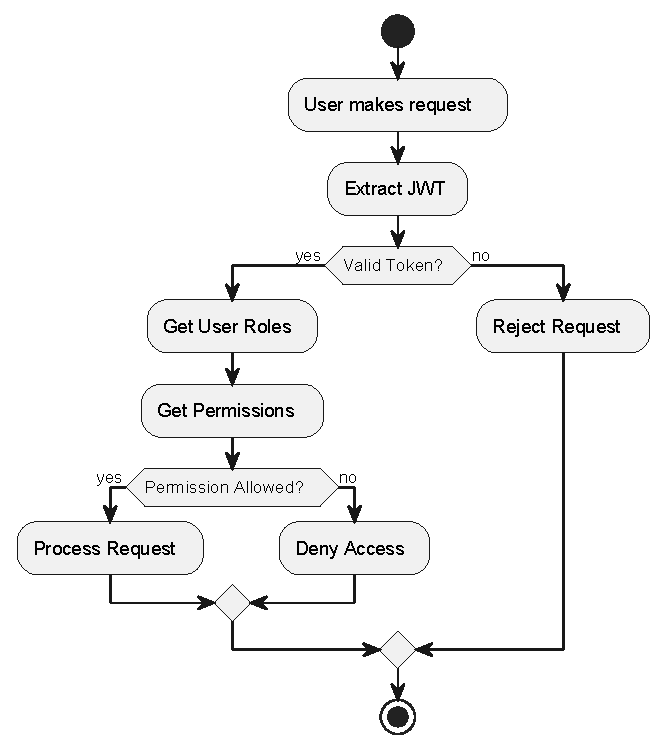
\includegraphics[width=0.95\textwidth]{figures/diagrams/activity_diagram_RBAC.pdf}
	\caption{Activity diagram: RBAC decision flow}
	\label{fig:activity-rbac}
\end{figure}

\section{Chapter Conclusion}
The modeling phase validates the structure of the proposed solution and makes the implementation task more explicit. By separating dynamic behavior, static structure, and data organization, the chapter demonstrates that MapIT has been designed in a disciplined way. The next chapter explains how this design was realized in the actual software stack.
